\documentclass{beamer}
\setbeamertemplate{footline}[page number]
\date{}
\author{}
\institute{}

%%%%%%% Put these names back in the final version 
%\\Aswathy Rajendra Kurup\\Meenu Ajith}
%\institute{Department of Electrical and Computer Engineering\\The University of New Mexico}
\setbeamercovered{transparent}
\usepackage{setspace}
\usepackage{array}
\usepackage[T1]{fontenc}
\usepackage{graphicx}
\usepackage{amsmath}
\usepackage{amsfonts}
\usepackage{amssymb}
\usepackage{makeidx}
\usefonttheme{serif}
\usepackage{multirow}
\usepackage{booktabs} 
\usepackage{rotating}
\usepackage{color}
\usepackage{float}
\usepackage[latin1]{inputenc}
\usepackage[english]{babel}
\usepackage{amsmath}
\usepackage{amsfonts}
\usepackage{eurosym}
\usepackage{rotating}
\usepackage{multicol}
\usepackage{pythonhighlight}
\usepackage[normalem]{ulem}
\newcommand{\ba}{{\bf a}}
\newcommand{\bb}{{\bf b}}
\newcommand{\bc}{{\bf c}}
\newcommand{\bd}{{\bf d}}
\newcommand{\be}{{\bf e}}
\newcommand{\bbf}{{\bf f}}
\newcommand{\bg}{{\bf g}}
\newcommand{\bh}{{\bf h}}
\newcommand{\bi}{{\bf i}}
\newcommand{\bk}{{\bf k}}
\newcommand{\bl}{{\bf l}}
\newcommand{\bm}{{\bf m}}
\newcommand{\bn}{{\bf n}}
\newcommand{\bo}{{\bf o}}
\newcommand{\bp}{{\bf p}}
\newcommand{\bq}{{\bf q}}
\newcommand{\br}{{\bf r}}
\newcommand{\bs}{{\bf s}}
\newcommand{\bt}{{\bf t}}
\newcommand{\bu}{{\bf u}}
\newcommand{\bv}{{\bf v}}
\newcommand{\bw}{{\bf w}}
\newcommand{\bx}{{\bf x}}
\newcommand{\by}{{\bf y}}
\newcommand{\bz}{{\bf z}}

\newcommand{\bA}{{\bf A}}
\newcommand{\bB}{{\bf B}}
\newcommand{\bC}{{\bf C}}
\newcommand{\bE}{{\bf E}}
\newcommand{\bG}{{\bf G}}
\newcommand{\bH}{{\bf H}}
\newcommand{\bI}{{\bf I}}
\newcommand{\bK}{{\bf K}}
\newcommand{\bL}{{\bf L}}
\newcommand{\bM}{{\bf M}}
\newcommand{\bO}{{\bf O}}
\newcommand{\bQ}{{\bf Q}}
\newcommand{\bR}{{\bf R}}
\newcommand{\bS}{{\bf S}}
\newcommand{\bT}{{\bf T}}
\newcommand{\bV}{{\bf V}}
\newcommand{\bW}{{\bf W}}
\newcommand{\bX}{{\bf X}}
\newcommand{\bY}{{\bf Y}}
\newcommand{\bZ}{{\bf Z}}
\newcommand\uptocnt{\stackrel{\mathclap{\normalfont\mbox{c}}}{\propto}}
\newcommand{\bpt}{{\bf pt}}
\newcommand{\bpl}{{\bf pl}}
\newcommand{\bdp}{{\bf dp}}
\newcommand{\btemp}{{\bf temp}}

\newcommand{\bmu}{{\boldsymbol \mu}}
\newcommand{\bSigma}{{\boldsymbol \Sigma}}
\newcommand{\bsigma}{{\boldsymbol \sigma}}
\newcommand{\bvarPhi}{{\boldsymbol \varPhi}}
\newcommand{\bvarphi}{{\boldsymbol \varphi}}
\newcommand{\bPhi}{{\boldsymbol \Phi}}
\newcommand{\bdelta}{{\boldsymbol \delta}}
\newcommand{\bZero}{{\bf 0}}
\newcommand{\bOne}{{\bf 1}}
\newcommand{\balpha}{{\boldsymbol \alpha}}
\newcommand{\bAlpha}{{\boldsymbol A}}
\newcommand{\btheta}{{\boldsymbol \theta}}

\newcommand{\softmax}{\text{softmax}}
\newcommand{\diag}{\text{diag}}
\newcommand{\sinc}{\mathrm{sinc}}
\newcommand{\argmin}{\mathop{\mathrm{argmin}}}
\newcommand{\infl}{\eta}
\newcommand{\Ind}{\mathrm{I}}
\newcommand{\Real}{\mathbb R}
\newcommand{\Intg}{\mathbb Z}
\newcommand{\Complex}{\mathbb C}
\newcommand{\Natural}{\mathbb N}
\newcommand{\Fourier}[1]{\mathcal{F} \{#1\}}
%\newcommand{\ii}{\mathbbm{i}}
\newcommand{\bphi}{\boldsymbol{\mathit{\phi}}}

\newcommand{\hs}{\hspace{2pt}}
\newcommand{\sign}{\text{sign}}
\author{Manel Mart\'inez-Ram\'on\\Meenu Ajith\\Aswathy Rajendra Kurup}

\usetheme{Madrid}
\usecolortheme{beaver}
\usepackage{tikz}
\usetikzlibrary{fit,arrows,calc,positioning}
\usepackage{listings}
\usepackage{xcolor}
\usepackage{emerald} 
\usepackage[T1]{fontenc} 
\usepackage{verbatim}
\usepackage{graphicx}
\usepackage{epsfig}
\usepackage{psfrag}
\usepackage[english]{babel}
\usepackage{listings}
\usepackage{courier}
\usepackage{color}
 \usepackage{vwcol} 
 \usepackage[english]{babel} % To obtain English text with the blindtext package
\usepackage{blindtext}
\definecolor{codegreen}{rgb}{0,0.6,0}
\definecolor{codegray}{rgb}{0.5,0.5,0.5}
\definecolor{codepurple}{rgb}{0.58,0,0.82}
\definecolor{backcolour}{rgb}{0.95,0.95,0.92}

\lstdefinestyle{mystyle}{
  backgroundcolor=\color{backcolour},   commentstyle=\color{codegreen},
  keywordstyle=\color{magenta},
  numberstyle=\tiny\color{codegray},
  stringstyle=\color{codepurple},
  basicstyle=\ttfamily\footnotesize,
  breakatwhitespace=false,         
  breaklines=true,                 
  captionpos=b,                    
  keepspaces=true,                 
  numbers=left,                    
  numbersep=5pt,                  
  showspaces=false,                
  showstringspaces=false,
  showtabs=false,                  
  tabsize=2
}
\lstset{style=mystyle}

%% Stuff for movies

% %\newcommand{\bt}{{\bf t}}
% \newcommand{\br}{{\bf r}}
% \newcommand{\bs}{{\bf s}}
% \newcommand{\by}{{\bf y}}
% \newcommand{\bz}{{\bf z}}
% \newcommand{\bx}{{\bf x}}
% \newcommand{\bw}{{\bf w}}
% \newcommand{\be}{{\bf e}}
% \newcommand{\bbf}{{\bf f}}
% \newcommand{\bb}{{\bf b}}
% \newcommand{\bd}{{\bf d}}
% \newcommand{\bA}{{\bf A}}
% \newcommand{\bB}{{\bf B}}
% \newcommand{\bL}{{\bf L}}
% \newcommand{\bM}{{\bf M}}

% \newcommand{\bC}{{\bf C}}
% \newcommand{\bI}{{\bf I}}
% \newcommand{\bK}{{\bf K}}
% \newcommand{\bk}{{\bf k}}
% \newcommand{\bT}{{\bf T}}
% \newcommand{\bV}{{\bf V}}
% \newcommand{\bW}{{\bf W}}
% \newcommand{\bX}{{\bf X}}
% \newcommand{\bY}{{\bf Y}}
% \newcommand{\bZ}{{\bf Z}}
% \newcommand{\bm}{{\bf m}}
% \newcommand{\bpt}{{\bf pt}}
% \newcommand{\bpl}{{\bf pl}}
% \newcommand{\bdp}{{\bf dp}}
% \newcommand{\btemp}{{\bf temp}}
% \newcommand{\bl}{{\bf l}}
% \newcommand{\bu}{{\bf u}}
% \newcommand{\bmu}{{\boldsymbol \mu}}
% \newcommand{\bSigma}{{\boldsymbol \Sigma}}
% \newcommand{\bLambda}{{\boldsymbol \Lambda}}

% \newcommand{\bsigma}{{\boldsymbol \sigma}}
% \newcommand{\bvarphi}{{\boldsymbol \varPhi}}
% \newcommand{\btheta}{{\boldsymbol \theta}}
% \newcommand{\bZero}{{\bf 0}}
% \newcommand{\balpha}{{\boldsymbol \alpha}}
% \newcommand{\bpi}{{\boldsymbol \pi}}
% \newcommand{\bxi}{{\boldsymbol \xi}}
% \newcommand{\bdelta}{{\boldsymbol \delta}}
\lstset{
	language=Python,
	basicstyle=\footnotesize\ttfamily\color{black},
	commentstyle = \footnotesize\ttfamily\color{red},
	keywordstyle=\footnotesize\ttfamily\color{blue},
	stringstyle=\footnotesize\ttfamily\color{black},
%	columns=fixed,
%	numbers=left,    
	numberstyle=\tiny,
	stepnumber=1,
	numbersep=5pt,
	tabsize=1,
	extendedchars=true,
	breaklines=true,            
	frame=b,         
	showspaces=false,
	showtabs=true,
	xleftmargin=6pt,
	framexleftmargin=6pt,
	framexrightmargin=2pt,
	framexbottommargin=4pt,
	showstringspaces=false      
}

\lstloadlanguages{
         Python
}

%\graphicspath{ {./images/} }  % Figures path - used in graphicx

%\selectcolormodel{cmyk}

\mode<presentation>

\newcommand{\dred}{darkred!90!black}
\newcommand{\written}{\ECFJD\textcolor{cyan!50!white}}
\newcommand{\hlight}{\textcolor{\dred}}
\newcommand{\Ex}{\textcolor{\dred}{Ex. }}

% remove navigation symbols in full screen mode
\setbeamertemplate{navigation symbols}{}  
\setbeamertemplate{blocks}[rounded][shadow=false]
\setbeamercolor{note page}{fg=black}

\setbeamercolor{title}{fg=\dred}
\setbeamercolor{frametitle}{fg=white}
\setbeamercolor{frametitle}{bg=\dred}
\setbeamercolor{structure}{fg=black,bg=white}
\setbeamercolor{background canvas}{bg=white,fg=black}
\setbeamercolor{normal text}{fg=black,bg=white}
\setbeamercolor{item}{fg=red!80!black,bg=white!}
\addtobeamertemplate{block begin}{\setbeamercolor{block title}{fg=white,bg=\dred}
\setbeamercolor{block body}{fg=white,bg=gray}}{}



%\title{Lesson 1.1}
\title{1. Feedforward neural networks }
\subtitle{1.2. Structure and optimization criteria}

\addtobeamertemplate{frametitle}{}


\begin{document}

\maketitle
\begin{frame}{Introduction}
\begin{itemize}
    \item The perceptron unit presented before is linear. 
    \item Nonlinear problems, as the classic XOR problem, cannot be solved with a perceptron. 
\end{itemize}
\begin{multicols}{2}
\begin{center}
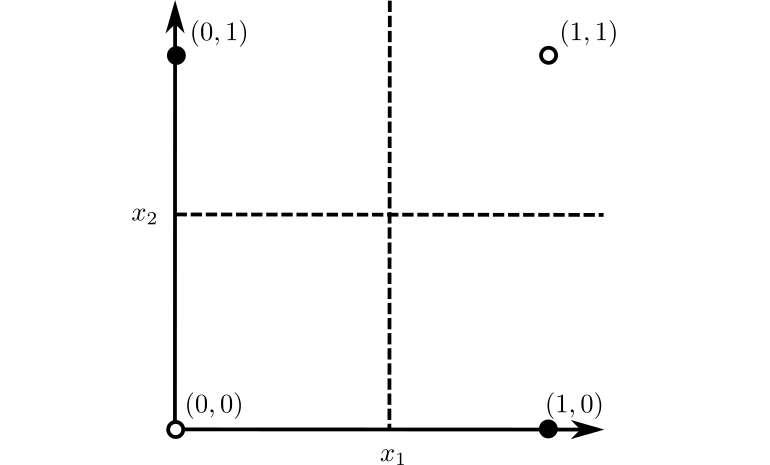
\includegraphics[scale=0.2]{Module 1 (NN)/pics/xor_problem.pdf}
\end{center}

\columnbreak

\begin{itemize}
\item The data labels are a XOR function of its coordinates: 
black dots are labelled with +1, white dots are labelled with 0.
\end{itemize}
\end{multicols}

\begin{itemize}
    \item A linear function cannot classify the data. It is possible to construct a nonlinear function with several perceptrons in two layers.
\end{itemize}

\end{frame}

\begin{frame}{Structure of a neural network}
\begin{multicols}{2}

    \begin{itemize}
\item  $L+1$ layers, layer $j=0$ is the input ${\bx}$ 
\item $L-1$ {\it hidden} layers with $D_j$ nodes with outputs $\bh^{(j)}$. 
\item The last layer implements the output $\bo$. 
\item Layers interconnected by linear weights  $\bW^{(j)}$. 
\end{itemize}





\centering
\includegraphics[scale=0.35]{pics/f4.1.pdf}

\end{multicols}


\end{frame} 

\begin{frame}{Structure of a neural network}

\begin{itemize}
\item The layers are interconnected by edges. Each edge contains a weight $w^{(l)}_{i,j}$ that connects the output of node $i$ of layer $l-1$ to the input of node $j$ in layer $l$. Also, each node has a bias input $b^{(l)}_j$.\\
\item Each node contains an affine transformation of the output of the previous layer as
\begin{equation}
    z^{(l)}_j=\sum_{i=1}^{D_{l-1}} w_{i,j}^{(l)} h^{(l-1)}_{i}+b^{(l)}_{j}={\bw_j^{(l)}}^\top  \bh^{(l-1)}+b_j^{(l)} 
\end{equation}

\item The output $j$ of layer $l$, $h^{(l)}_j$ is 
\begin{equation}\label{eq:unit}
    h^{(l)}_j = \phi\left(z^{(l)}_j \right) = \phi\left({\bw^{(l)}_j}^\top  \bh^{(l-1)}+b^{(l)}_j\right) 
\end{equation}
\end{itemize}
\end{frame}

\begin{frame}{A neuron}
\begin{multicols}{2}

    \begin{center}
    
\includegraphics[scale=0.35]{Module 1 (NN)/pics/neuron.pdf}
    \end{center}

Remarks:
\begin{itemize}
\item $b^{(l)}_j$ implements the bias. 
\item In some notations,  $b^{(l)}_j=w_{0,j}^{(l)}$ and $h^{(l-1)}_0=1$.
\item Element $w_{i,j}^{(l)}$ of vector $\bw_{j}^{(l)}$ represents the connection of node $i$ of layer $l-1$ with node $j$ of layer $l$.

\end{itemize}
\end{multicols}
\begin{itemize}
    \item The nonlinear activation for a hidden layer is not usually a sigmoidal, as we will see further. 
\end{itemize}
\end{frame}

\begin{frame}{Notation conventions}
    The following general notation conventions are taken in this course:
    \begin{itemize}
        \item Lowercase, normal letters as $b, w$ represent scalars, i.e. $b \in \mathbb{R}$.
        \item Uppercase normal letters as $D, N$ represent constants. 
        \item Lowercase bold letters as $\bb, \bw$ are column vectors. 
        \item Uppercase bold letters as $\bW$ are arrays. In this module, they are all 2D matrices, i.e, for example, $\bW \in \mathbb{R}^{D_1\times D_2}$ is a matrix of $D_1$ rows and $D_2$ columns. In general, an array may have more than 2 dimensions. 
    \end{itemize}
\end{frame}

\begin{frame}{Notation conventions}
The following conventions particular to the structure of neural networks are taken:
\begin{itemize}
    \item Superindex $(l)$ between parenthesis refer to output layers. $\bW^{(l)}$ refers to a matrix of weights that connects layer $l-1$ to layer $l$.
    \item Subindex $i$ in vector $\bw_i^{(l)}$ mean that this vector is the $i$-th column of matrix $\bW^{(l)}$. $\bw_i^{(l)}$ is then a \emph{column vector}.
    \item $\bb^{(l)}$ is a \emph{column vector} containing all the biases of layer $l$.
    \item Subindexes $i,j$ in scalar $w^{(l)}_{i,j}$ mean, equivalently, that:
    \begin{itemize}
        \item $w^{(l)}_{i,j}$ is the connection between node $i$ of layer $l-1$ and node $j$ of layer $l$.
        \item $w^{(l)}_{i,j}$ is $i_th$ element of vector $\bw^{(l)}_j$
        \item $w^{(l)}_{i,j}$ is element ${i,j}$ of matrix $\bW^{(l)}$.
        
    \end{itemize}    
\end{itemize}
    
\end{frame}




\begin{frame}{Activations for hidden nodes}
\begin{itemize}
\item The first activation for hidden nodes to be used was the sigmoid $$
    \sigma(z)=\frac{1}{1+e^{-z}} 
$$
\item Modern neural networks use the so-called rectified linear unit (ReLU)
\begin{equation}
    \phi(z) = \max(0,z) 
\end{equation}
\item ReLU is enough to provide the NN with nonlinear properties. 
\item A nonzero gradient extension of the ReLU is 
\begin{equation}
\phi(z_i)=max\{0,z_i\} + \alpha_i min\{0,z_i\}
\end{equation}
\end{itemize}
\end{frame}



\begin{frame}{Rectified Linear Units}



\begin{itemize}
\item Three versions of this activation are extremely useful. 
\begin{itemize}
    \item \emph{Absolute value} $\phi(z_i,\alpha_i)=max\{0,z_i\}- min\{0,z_i\}=|z_i|$
    \item  \emph{Leaky ReLU}, for small values of $\alpha_i$
    \item   \emph{Parametric ReLU} or PReLU,  when $\alpha_i$ is learnable using gradient descent. 
\end{itemize}

\begin{center}
\includegraphics[scale=0.4]{Module 1 (NN)/pics/ReLU.pdf}\\
\tiny{Left: Rectified Linear Unit (ReLU). Right: Leaky ReLU.}
\end{center}
    

\item Maxout units  divide ${\bf z}$ in groups of k elements, outputs the maximum 
\begin{equation}
\phi(z)_i=\max_{j\in G^{i}}(z_j)
\end{equation}
\item Maxout units can generalize any of the above activations. 
\end{itemize}

\end{frame}
 



\begin{frame}{Training criterion: Maximum Likelihood}
\begin{itemize}
\item Assume a dataset $\{{\bf x}_i,{\bf y}_i\}$, $1 \leq i \leq N$. If training outputs $\by_i$ are independent given their corresponding inputs $\bx_i$, the joint likelihood is equal to the product of likelihoods, this is 
\begin{equation}
    p(\bY|\bX) = \prod_i p(\by_i|\bx_i)
\end{equation}

\item Applying logarithms and dividing by the number of training data $N$ 
\begin{equation}\label{eq:cross_entropy_cost}
J_{ML}({\boldsymbol \theta})=-\frac{1}{N}\log p(\bY|\bX) = -\frac{1}{N}\sum_i \log  p(\by_i|\bx_i) \approx -\mathbb{E}_{{\bf x},{\bf y}} \log p({\bf y}|{\bf x})
\end{equation}
where $\theta$ represents the set of parameters $w^{(l)}_{j,k}$, $b_{k}^{(l)}$ to optimize.  
\item This is the cross entropy between the real and predicted probabilities (as we will see later). 
\end{itemize}
\end{frame}

\begin{frame}{Regularization}
\begin{itemize}
\item In order to minimize overfitting, many approaches use a regularization factor in the cost function that minimizes the square norm of the parameters, such as 
\begin{equation}\label{eq:reg_cross_entropy}
J(\boldsymbol \theta) = J_{ML}(\boldsymbol \theta) + \lambda \sum_{l} ||{\bf W}^{(l)}||_F^2
\end{equation}
where $||\cdot||^2_F$ is the squared Frobenius norm operator.
\begin{equation}
    ||{\bf W}^{(l)}||_F^2 = \sum_{j,k} w^2_{j,k}
\end{equation}
\item Other forms of regularization as dropout, early stopping or data augmentation will also be discussed. 
\end{itemize}
\end{frame}

\begin{frame}{Posterior distributions}
\begin{itemize}
\item Depending on the posterior distribution that we choose, the interpretation and the uses will be different. We will primarily use
\begin{itemize}
    \item Gaussian posterior for regression
    \begin{equation}
p({\bf y}|{\bf x})=\frac{1}{(2\pi)^{D/2}|{\boldsymbol \Sigma}|^{1/2}} e^{\left(-\frac{1}{2}\left({\bf y}- \bz\right)^{\top}{\boldsymbol \Sigma}^{-1}\left({\bf y}- \bz\right)\right)}
\end{equation}
    \item Sigmoid activation for binary classification
    \begin{equation}
    p(y=1|{\bf x})=\frac{1}{1+e^{-yz}} 
\end{equation}
    \item Softmax activations for multiclass classification
    \begin{equation}\nonumber
 p\left(y=k|{\bf x}\right)=\frac{e^{z_k}}{\sum_{j=1}^K e^{(z_{j})}}
\end{equation}
\end{itemize}
\end{itemize}
\end{frame}

\begin{frame}{Gaussian posterior for regression}
\begin{itemize}
\item Interpreted as a regression model with linear  output.  
\item The estimation error components are considered independent 
\begin{equation}
p({\bf y}|{\bf x})=\frac{1}{(2\pi \sigma^2)^{D/2}} \exp\left(-\frac{1}{2\sigma^2}||{\bf y}- \bz||^2\right)
\end{equation}
    
    
\item The cost function in Eq. \eqref{eq:cross_entropy_cost} for this model is
\begin{equation}\nonumber
\begin{split}
&J_{ML}({\boldsymbol \theta})=-\mathbb{E}_{{\bf x},{\bf y}} \log p({\bf y}|{\bf x})%\\&
=\mathbb{E}_{{\bf x},{\bf y}} \left(\frac{1}{2\sigma^2}\|{\bf y}- \bz\|^2+ \frac{D}{2} 2 \pi \sigma^2 \right)\\
& = \mathbb{E}_{{\bf x},{\bf y}} \left(\|{\bf y}- \bz\|^2 \right) +\text{constant}
\approx\frac{1}{N}\sum_{i=1}^N \|{\bf y}_i- {\bW^{(L)}}^\top{\bf h}^{(L-1)}\|^2 
\end{split}
\end{equation}
\end{itemize}
The output $\bz$ and the regressors $\by$ are assumed to be vectors (multitask regression).
\end{frame}

\begin{frame}{Sigmoid posterior for binary classification}
\begin{itemize}
\item We assume an unnormalized log-likelihood as 
\begin{equation}
\log \tilde{p}(y|{\bf x})=yz \longrightarrow \tilde{p}(y|{\bf x})=e^{yz}
\end{equation}
which must be normalized as 
\begin{equation}
    p(y|{\bx})=\frac{e^{yz}}{\sum_{y'=0}^1 e^{yz}}=\frac{e^{yz}}{1 + e^{z}}
\end{equation}
\item Therefore 
\begin{equation}
    \begin{split}
        p(y=0|\bx) & = \frac{1}{1+e^z}\\
        p(y=1|\bx) & = \frac{e^z}{1+e^z}
    \end{split}
\end{equation}
\end{itemize}
\end{frame}

\begin{frame}{Sigmoid posterior for binary classification}
\begin{itemize}
\item Since the sigmoid function is $\sigma(a)=\frac{1}{1+e^{-a}}$, then 


\begin{equation}
 p(y|{\bf x})=\frac{1}{1+e^{-(2y-1)z}}
 =\begin{cases}
 \frac{1}{1+e^z}, & y=0\\
 \frac{1}{1+e^{-z}}=\frac{e^z}{1+e^{z}}, & y=1\\
 \end{cases}
\end{equation}
\item Finally

\begin{equation}
 p(y|{\bf x})=\sigma\left( (2y-1){\bw^{(L)}}^\top  \bh^{(L-1)} \right)
\end{equation}


\item According to Eq. \eqref{eq:cross_entropy_cost}, the cost function is
\begin{equation}\label{eq:bernoulli_cost_function}
J_{ML}(\boldsymbol \theta)=\mathbb{E}\left[\log \sigma((2y-1)z)\right]=-\mathbb{E}\left[ \log\left(1+e^{(1-2y)z}\right)\right]
\end{equation}
\end{itemize}
\end{frame}

%\begin{frame}{Sigmoid posterior for binary classification}
%\begin{center}
%\includegraphics[scale=0.37]{pics/f4.5.pdf}
%\end{center}
%\small{Cross entropy cost function (blue) and MSE cost function (red) for the Bernoulli log likelihood for a single sample with $y=1$. The cross entropy cost function has a derivative that increases when the value of the function increases. The MSE cost function has a very small derivative when the function tends to its maximum.}
    
%\end{frame}

\begin{frame}{Softmax posterior for multiclass classification}
\begin{itemize}
    \item 
Here the neural network has a vectorized output 
\begin{equation}
{\bf z}={{\bf W}^{(L)}}^{\top}{\bf h}^{(L-1)}
\end{equation}

    
\item Then, we model each element $z_k$ in $\bf z$ as 
\begin{equation}
\begin{split}
z_k&=\log \tilde{p}(y=k|{\bf x})\\
\tilde{p}(y=k|{\bf x})&=e^{z_k}
\end{split}
\end{equation}

and then we normalize  \emph{softmax} function, 
\begin{equation}\label{eq:softmax}
p(y=k|{\bf x})=\text{softmax}(z_k)=\frac{e^{z_k}}{\sum_{j=1}^K e^{z_j}}
\end{equation}
\end{itemize}
\end{frame}


\begin{frame}{Softmax posterior for multiclass classification}

\begin{itemize}
    \item The log-likelihood function can be interpreted as a cross-entropy between the actual probability of the label and the estimated one:
    \begin{equation}
    H(q,p) = -\mathbb{E} \left[q \log p \right]
    \end{equation}
    For the binary case, the equivalence is straightforward (exercise).
    
    \item For the multiclass case:
    \begin{enumerate}
        \item We first change the multiclass label $y_i =k$, $1\leq k \leq K$ by a vector $\by_i=\left[ y_i^{(1)},\cdots,y_i^{(K)}  \right]$ where $y_i^{(k)}=1$ and the rest are zero.
        \item We denote the real probability that $y_i=k$ as 
        \begin{equation}
            q\left(y_i^{(k)}=1\right) = q_i(k) = \begin{cases}
            1, & y_i=k\\
            0, & y_i \neq k
            \end{cases}
        \end{equation}
    \end{enumerate}
    
\end{itemize}
\end{frame}

\begin{frame}{Softmax posterior for multiclass classification}
\begin{itemize}
\item The cross-entropy loss for sample $i$ can be written as 
\begin{equation}
\ell_i = -\sum_{k=1}^{K} q_y(k) \log p(y_i=k|\bx)      
\end{equation}
\item Note that  $q_i(k)=y^{(k)}_i$. By changing  $p(y_i=k|\bx) $ by Eq. \eqref{eq:softmax}

\begin{equation}\label{eq:cross_entropy1}
    l_i=-\sum_{k=1}^{K} y_i^{(k)} \log\frac{e^{z_{i,k}}}{\sum_{j=1}^{K} e^{z_{i,j}}}
    =-\sum_{k=1}^{K} y_i^{(k)} z_{i,k} +\sum_{k=1}^{K} y_i^{(k)}\log \sum_{j=1}^{K} e^{z_{i,j}}
\end{equation}
\item Since only one of the elements of vector $\by_i$ is 1
\begin{equation}\label{eq:cross_entropy2}
l_i=-\sum_{k=1}^{K} y_i^{(k)} z_{i,k} + \log \sum_{j=1}^{K} e^{z_{i,j}}\end{equation}
where $z_{i,k}$ is the $k$-th output for input sample $\bx_i$.
\end{itemize}
\end{frame}
	

 \end{document}
